\documentclass[tikz,border=0pt]{standalone}
\begin{document}
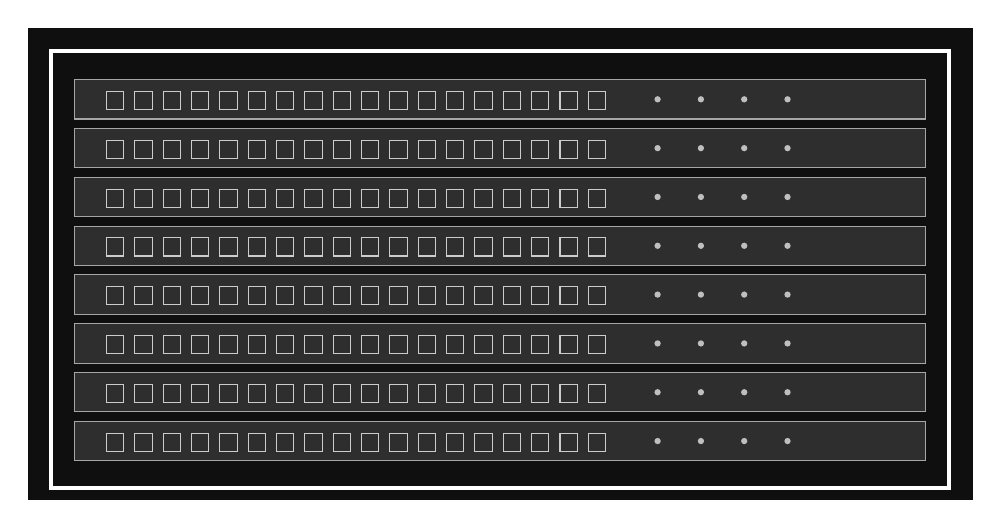
\begin{tikzpicture}
\fill[black!94] (0,0) rectangle (12,6);
\foreach \i in {0,...,7}{
  \fill[black!82] (.6,.5+\i*.62) rectangle (11.4,1+\i*.62);
  \draw[white!65!black] (.6,.5+\i*.62) rectangle (11.4,1+\i*.62);
  \foreach \j in {0,...,17}{
    \draw[white!80!black] (1+\j*.36,.62+\i*.62) rectangle (1.22+\j*.36,.85+\i*.62);}
  \foreach \j in {0,...,3}{\fill[white!75!black] (8+\j*.55,.75+\i*.62) circle (.04);}
}
\draw[white,line width=1.5pt] (.3,.15) rectangle (11.7,5.7);
\end{tikzpicture}
\end{document}
